\documentclass[../main.tex]{subfiles}

\begin{document}

\chapter{Quantum Systems}
\label{sec:sevenfive}


\section{Hydrogen molecule}
\subsection{Finding the ground state energy using VarITE}
The Hydrogen Hamiltonian of the Hydrogen molecule transformed using the Bravely-Kitaev transformation and a bond length of $R=0.75$ \cite{McArdle_2019} goes as follows:
\begin{equation*}
H=0.2252 I+0.3435 Z_{0}-0.4347 Z_{1}+0.5716 Z_{0} Z_{1}+0.0910 Y_{0} Y_{1}+0.0910 X_{0} X_{1}
\end{equation*}
The ansatz can be seen in \autoref{fig:H2_ansatz}
\begin{figure}[h]
    \begin{center}
        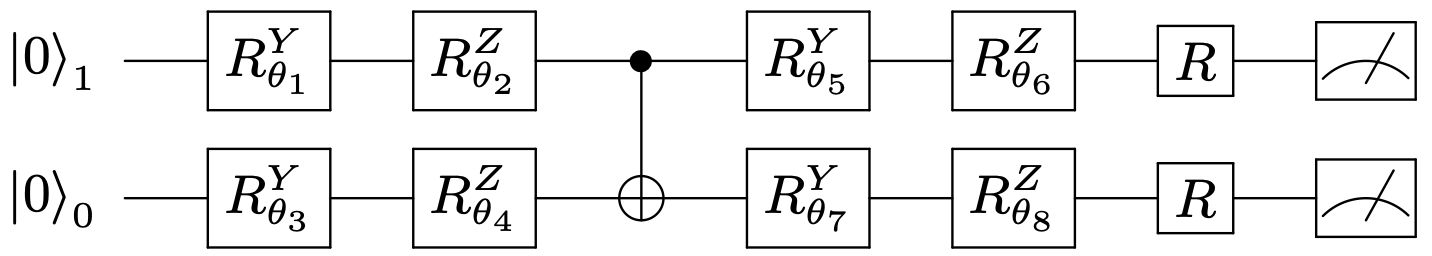
\includegraphics[scale=0.45]{figures/ansatz_varite.png}
        \caption{Ansatz used to find the ground state energy. The $R$ gates represent the rotational gates depending on the basis of measurement}
        \label{fig:H2_ansatz}
    \end{center}
\end{figure}

Finding the  grounds state energy of a hydrogen molecule using VarITE and different initialisations of the ansatz parameters can been seen in \autoref{fig:H2_distribution}.

\begin{figure}
    \begin{center}
        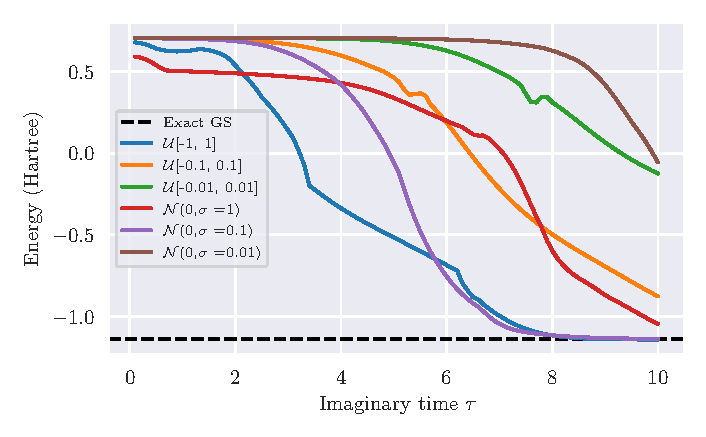
\includegraphics{figures/energy_H2_search_01step.pdf}
        \caption{Energy as a function of imaginary time using different distributions}
        \label{fig:H2_distribution}
    \end{center}
\end{figure}

Using a distribution of $\N(0,\sigma=0.1)$, the ground state energy were found using different step sizes. The figure can be seen in \autoref{fig:H2_step}

\begin{figure}
    \begin{center}
        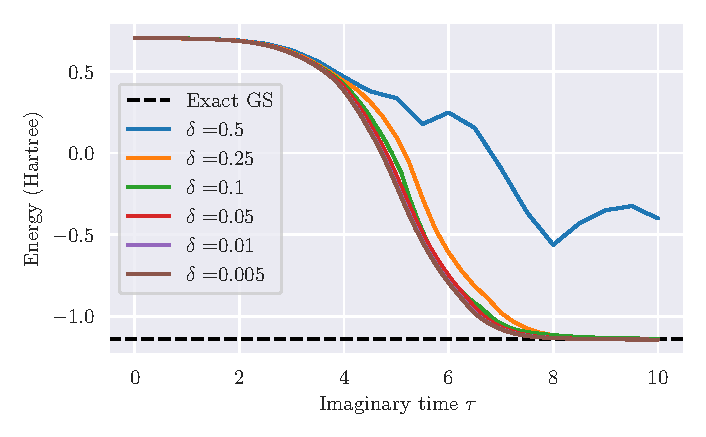
\includegraphics{figures/energy_H2_search_N01.pdf}
        \caption{Energy as a function of Energy as a function of imaginary time for different sizes of time steps.}
        \label{fig:H2_step}
    \end{center}
\end{figure}
\subsection{Finding the ground state energy using RBM}
The Restricted Boltzmann machine where used with neural-network quantum states was utilized to find the ground state energy of the $H_2$ molecule with a bond length of $1.40$ Bohr radii. Doing a parameter search of the fixed variance $\sigma$ of the NQS can be seen in figure \autoref{fig:sigmarbm}

\begin{figure}
    \begin{center}
        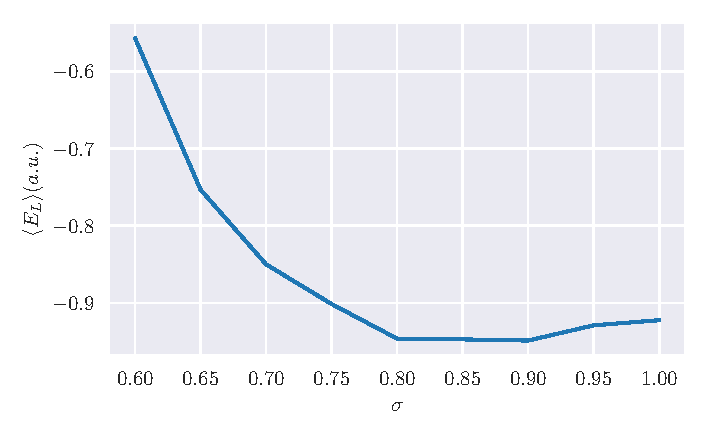
\includegraphics{figures/sigma_investigation.pdf}
        \caption{Energy as function of $\sigma$}
        \label{fig:sigmarbm}
    \end{center}
\end{figure}

The chosen value of $\sigma$ was set to $0.9$ for future computations. The learning rate $\gamma$ were seen to affect the results fairly little with $\gamma \in [10^{-3}, 10^{-1}]$, therefore the learning rate was set to $0.01$. The number of hidden nodes were then investigated for a variety of hidden nodes. The final results can be seen in \autoref{tab:rbm_hid_h2}

Further on the

\begin{table}[H]
\centerline{
\begin{tabular}{ ccccc } 
\toprule
Hidden Nodes & E_{C}(\ensuremath{a.u}) & \ensuremath{\mu}_{C} & E_{ref}(\ensuremath{a.u})& Dissimilarity\\ 
\midrule
 2 & -0.952 & 2.9\cdot10^{-3} & −1.1746 & 18.94\\
 \textbf{5} & \textbf{-0.955} & \textbf{2.9}\mathbf\cdot\mathbf{10^{-3}} & \textbf{−1.1746} & \textbf{18.71}\\
 10 & -0.951 & 2.9\cdot10^{-3} & −1.1746 & 19.03\\
 20 & -0.946 & 2.8\cdot10^{-3} & −1.1746 & 19.45\\
\bottomrule
\end{tabular}}
\caption{Local energies of the $H_2$ molecule with a bond length of 1.40 Bohr radii, utilizing 50 RBM cycles and $2^{18}$ Gibbs steps. The standard deviation \ensuremath{\mu} was computed using the blocking method. The subscript $C$ and $ref$ stands for computed and referenced. The reference value represents the experimental ground state energy.}
\label{tab:rbm_hid_h2}
\end{table}



\end{document}